\documentclass[preprint,12pt,authoryear]{elsarticle}
\usepackage{amsmath,amsfonts}
\usepackage{algorithmic}
\usepackage{algorithm}
\usepackage{array}
\usepackage{booktabs}
\usepackage{multirow}
\usepackage{textcomp}
\usepackage{url}
\usepackage{graphicx}
\usepackage{tikz}
\usepackage{enumitem}
\usepackage{lineno}
\usepackage{placeins}
\usepackage[export]{adjustbox}
\usetikzlibrary{fit,backgrounds,calc}
\usepackage{pgfplots}
\usepgfplotslibrary{groupplots}
\pgfplotsset{compat=1.16}
\newcommand{\modl}[1]{{\tiny\ttfamily #1}}
\setlength{\emergencystretch}{3em}
\renewcommand{\_}{\textunderscore\allowbreak{}}
\usetikzlibrary{arrows.meta, positioning, shapes.geometric}
\journal{Journal of Systems and Software}
\modulolinenumbers[5]

\begin{document}

\begin{frontmatter}

\title{CADENCE: Case-Grounded, Deliberation-Driven, and Solver-Verified Architectural Decision-Making with Large Language Models}

\author{Quang-Vinh Dang}
\ead{vinh.dq4@buv.edu.vn}
\address{British University Vietnam, Hung Yen, Vietnam}

\begin{abstract}
Large language models (LLMs) are increasingly proposed as assistants for architectural decision-making, yet most existing approaches either generate an architecture decision record (ADR) from a single unconstrained LLM call, retrieve similar precedents without reconciling the competing quality-attribute concerns a real decision must balance, or debate among multiple agents without any formal check that the resulting decision is realizable within a bounded budget of architectural tactics. We present CADENCE, a four-stage algorithm combining (1) retrieval-augmented case-based reasoning over a corpus of real, mined ADRs, (2) knowledge-graph-grounded multi-agent deliberation in which each agent advocates for one ISO/IEC~25010-derived quality attribute, (3) constraint-solver-verified feasibility, encoded as a two-phase weighted MaxSAT/SMT problem in Z3 and repaired via an LLM-driven loop targeting the solver's uncovered-attribute signal (its unsatisfiable core is reported only as a supplementary diagnostic), and (4) a separate self-critique pass blending a deterministic structural utility score with a qualitative LLM judgment. Unlike prior multi-agent architectural decision systems, whose agents occupy sequential functional roles and whose ``evaluation'' step is itself another LLM opinion, CADENCE's agents represent adversarial quality-attribute concerns and its feasibility check is a formal solver, not a second language model. We implement the full pipeline against a real corpus of 6{,}173 mined ADRs and evaluate it on two independently-sampled held-out sets ($N=3$ each, real end-to-end local-model wall-clock cost being the binding constraint on sample size) against four baselines forming an ablation ladder --- zero-shot generation, retrieval-only generation, multi-agent deliberation without solver verification, and CADENCE without self-critique --- on BERTScore, BLEU, ROUGE-1, and METEOR, plus two metrics only a solver-verified system can report: constraint-satisfaction rate and repair-loop convergence. At the one tested budget where feasibility is arithmetically possible ($B=5$), constraint satisfaction is 0\% and repair never converges even with its full design budget --- an honest negative result we diagnose mechanistically rather than soften; the tighter budgets we also test are infeasible by construction and reported only as construction checks. Against this, self-critique shows a modest but consistent positive signal: CADENCE with self-critique scores higher than without it in 7 of 8 system-budget-metric comparisons, the only ablation where adding a stage helps rather than being flat. We separately find surface n-gram metrics penalize CADENCE's deliberately terse, solver-parseable output relative to baselines prompted for open-ended prose, while BERTScore remains comparable across all systems; we argue this is an asymmetry, not a quality gap, with implications for evaluating structured multi-stage LLM pipelines generally. Beyond our own re-implemented baselines, we locate our exact held-out items within a public replication package's real, published generations from four frontier models and compare directly against them, giving an external reference point our baselines alone cannot provide.
\end{abstract}

\begin{keyword}
Large language models \sep architectural decision-making \sep architecture decision records \sep multi-agent systems \sep constraint solving \sep retrieval-augmented generation \sep self-critique \sep software architecture
\end{keyword}

\end{frontmatter}

\linenumbers

\section{Introduction}

Software systems accumulate architectural decisions continuously: how to scale a read-heavy component, whether to introduce a message queue, where to draw a service boundary, how to trade encryption overhead against latency. Each such decision commits a team to consequences across multiple, frequently conflicting quality attributes --- performance against maintainability, scalability against cost, security against usability --- and each is, in practice, made under time pressure, with incomplete visibility into precedent, and without a systematic check that the chosen tactics are mutually consistent within what the team can actually staff and afford. Architecture decision records (ADRs) exist to make this reasoning explicit and reviewable, yet writing one well --- surveying precedent, weighing competing quality attributes on their merits, and verifying that the resulting commitments do not silently exceed what the team can deliver --- is exactly the kind of effortful reasoning that teams under delivery pressure are most likely to shortcut.

Large language models are a natural candidate to assist here, and a growing body of work explores LLM-assisted architectural decision-making and ADR generation. The most direct approaches prompt a single LLM, zero-shot or with light context, to draft a decision from stated requirements~\citep{dhar2024llm}. A second line grounds generation in retrieval over real, mined ADR corpora, anchoring output in precedent rather than parametric knowledge alone~\citep{contextmatters2026}. A third introduces multiple LLM agents, most notably a four-agent pipeline of functional roles --- an Analyst, a Modeler, a Designer, and an Evaluator --- each handling a different phase of the decision~\citep{maad2025}. Each line solves part of the problem this paper addresses, but none solves all of it, and none can answer a question that matters for any decision with real operational consequences: \emph{is the decision the model just wrote actually feasible, given a bounded, explicit budget of architectural commitments the team can realistically execute?} A single LLM call has no mechanism to check this. Retrieval grounds the decision in precedent but does not reconcile competing quality-attribute demands, let alone verify them formally. And a multi-agent pipeline whose final ``Evaluator'' step is itself another LLM call is still, ultimately, one model's opinion of another's output --- persuasive, perhaps, but not a proof of anything.

This paper presents CADENCE, a four-stage algorithm designed around this gap directly. CADENCE (1) retrieves precedent decisions from a real corpus of mined, human-authored ADRs via dense vector search, so deliberation starts from what teams have actually decided before, not a blank context window; (2) stages a bounded, structured multi-agent deliberation in which each agent is anchored to one ISO/IEC~25010-derived~\citep{iso25010} quality attribute --- performance, security, maintainability, scalability, and cost/operability --- and argues for the candidate decision that best serves its attribute, grounded in a knowledge graph of architectural tactics, so the competing concerns a real decision must balance are represented explicitly and adversarially rather than folded into one model's undifferentiated judgment, with the graph's cross-attribute trade-off structure carried forward into Stage~3's feasibility check and Stage~4's utility scoring; (3) encodes the deliberated candidate's implied tactic commitments as a two-phase weighted MaxSAT/SMT problem checked with the Z3 theorem prover, and, if infeasible under a caller-specified tactic budget, constructs a targeted repair prompt from the solver's uncovered-attribute signal (its unsatisfiable core, when available, is a supplementary diagnostic, not the repair driver) and issues it as a standalone repair call, iterating to a fixed cap and degrading gracefully with an explicit caveat if feasibility is never reached; and (4) finalizes the solver-verified decision through a separate self-critique pass combining a deterministic structural utility score --- derived from which quality attributes the selected tactics actually cover, and what trade-offs they incur --- with a qualitative LLM judgment of remaining weaknesses, so the system's confidence is never purely self-reported by the same reasoning process that produced the decision. Each stage closes a specific failure mode the others leave open: retrieval alone cannot reconcile competing quality attributes; deliberation alone cannot verify feasibility; and an unverified, unaudited decision cannot be trusted as final without an independent finalization pass.

We implement the complete CADENCE pipeline end-to-end against a real, publicly available corpus of 6{,}173 mined ADRs drawn from 882 open-source repositories~\citep{buchgeher2023adr}, and evaluate it against four baselines forming an ablation ladder, each adding exactly one stage over the previous: zero-shot generation, retrieval-only generation, multi-agent deliberation without solver verification, and CADENCE without self-critique (adds Stage~3's solver-verified feasibility and repair loop, but not Stage~4). This ladder isolates retrieval's, deliberation's, solver verification's, and self-critique's contributions individually. We report the standard generation-quality metrics used in prior ADR-generation work --- BERTScore, BLEU, ROUGE-1, and METEOR --- against held-out, human-authored ground truth, alongside two metrics only a solver-verified system can report: constraint-satisfaction rate and repair-loop convergence. Our results surface a methodologically important asymmetry: surface n-gram overlap metrics (ROUGE-1, METEOR) penalize CADENCE's deliberately terse, structured output --- terse by design, so Stages 3 and 4 can parse it reliably --- relative to baselines prompted for open-ended prose closer in length to the reference ADRs, while BERTScore, far less sensitive to this length mismatch, remains comparable across all four systems. We report this honestly rather than letting a metric artifact of our own prompt design misrepresent the comparison, and discuss what it implies for evaluating structured, multi-stage LLM pipelines whose intermediate representations are deliberately not free-form prose.

This work makes three contributions. First, CADENCE, to our knowledge the first architectural decision-making algorithm combining real-corpus retrieval, adversarial quality-attribute-grounded multi-agent deliberation, formal constraint-solver verification with a solver-in-the-loop repair mechanism, and a separately-scored self-critique finalization stage. Second, a concrete construction for turning free-text, LLM-authored deliberation into a solvable constraint-satisfaction instance, with one design choice empirically validated during development: a lexicographic, rather than weighted-sum, multi-objective optimization is required to make coverage strictly dominate trade-off avoidance regardless of caller-supplied weight magnitudes, a subtlety a naive encoding gets wrong (Section~\ref{sec:method-stage3}). Whether the full construction reliably reaches feasibility in practice is an open question our small-sample evaluation (Section~\ref{sec:evaluation}) does not yet settle --- we report a fully-diagnosed negative result rather than a positive one. Third, a real, if small-sample, empirical evaluation against real baselines on a real corpus --- including a direct comparison, on identical held-out items, against real published generations from four frontier models via an independent public replication package (Section~\ref{sec:published-comparison}) --- surfacing a metric asymmetry (BERTScore versus surface n-gram overlap) we believe generalizes to other structured, multi-stage LLM systems.

The remainder of this paper is organized as follows. Section~\ref{sec:related} positions CADENCE against the closest prior systems for LLM-assisted architectural decision-making and against the broader techniques it draws on. Section~\ref{sec:method} presents the CADENCE algorithm in full, stage by stage. Section~\ref{sec:evaluation} describes our experimental setup, baselines, metrics, and results. Section~\ref{sec:discussion} discusses limitations, threats to validity, and the metric-asymmetry finding. Section~\ref{sec:conclusion} concludes.

\section{Related Work}
\label{sec:related}

\subsection{LLM-Assisted Architectural Decision-Making}

\citet{dhar2024llm} demonstrate that a single LLM, prompted with a stated architectural problem, can produce a plausible ADR, but their approach neither retrieves precedent nor verifies the result against any formal notion of feasibility: the model's output is accepted as-is. Follow-on work from the same group frames ADR authoring as an explicit drafting process rather than one-shot generation~\citep{dhar2025drafting}, and a separate recent study evaluates LLMs specifically as \emph{detectors} of violations against already-recorded architectural decisions~\citep{su2026violations} --- a complementary, downstream concern rather than assisting the decision itself. A complementary line of work treats the growing body of real, mined ADRs as a resource in its own right: large-scale mining studies of ADR adoption in open-source projects~\citep{buchgeher2023adr} establish both the raw corpus this paper's retrieval stage draws on and the empirical observation --- corroborated in our own corpus statistics --- that ADR adoption per repository is sparse, which any retrieval-based system must tolerate rather than assume away. Building on such corpora, retrieval-grounded generation work~\citep{contextmatters2026,contextmatters-zenodo} shows that conditioning an LLM's ADR generation on retrieved precedent measurably improves output quality, and explicitly frames the task this paper's held-out evaluation also uses: given only a decision's title, generate the body. This precedent motivates our own held-out query construction (Section~\ref{sec:evaluation}) and supplies both the retrieval-only baseline and the corpus itself. Neither line of work, however, reconciles multiple quality-attribute concerns or checks feasibility formally --- gaps CADENCE is designed to close.

The closest prior system to CADENCE is MAAD~\citep{maad2025}, a four-agent pipeline in which an Analyst, a Modeler, a Designer, and an Evaluator agent each handle one sequential phase of the decision process; a related paper from an overlapping author group targets generating the \emph{rationale} behind an already-made decision rather than the decision itself~\citep{zhou2025rationale}. MAAD and CADENCE share the premise that a single LLM call is insufficient and multiple agents should participate, but the two systems differ in three load-bearing ways. First, MAAD's agents occupy sequential \emph{functional} roles --- each does a different \emph{kind} of work at a different pipeline point --- whereas CADENCE's agents occupy simultaneous, \emph{adversarial} roles: every agent does the same kind of work (propose and critique a candidate) but from a different, often conflicting quality attribute, so the tension between (e.g.) a performance-motivated tactic and its maintainability cost is an argument between agents rather than resolved silently inside one agent's reasoning. Second, MAAD's Evaluator is itself an LLM judge assessing the Designer's output with the same kind of model that produced it, so MAAD's final confidence is ultimately one language model's opinion of another's work. CADENCE's Stage~3 feasibility check is a formal constraint solver over an explicit tactic budget and coverage requirement; a decision either satisfies the encoded constraints or not, independent of any model's subjective assessment, and when it does not, the solver's uncovered-attribute signal gives the repair loop a structured target rather than generic revision instructions (the unsatisfiable core is also reported, as a supplementary diagnostic). Third, CADENCE's retrieval stage is grounded in a large, real, citable corpus of mined ADRs, giving deliberation a case-based starting point that MAAD's requirements-only formulation does not provide. We discuss MAAD further, and compare against a solver-free multi-agent ablation modeled directly on this difference, in Section~\ref{sec:evaluation}. Table~\ref{tab:relatedwork} summarizes this positioning.

\begin{table}[!htbp]
\caption{Positioning Against the Closest Prior LLM-Assisted Architectural Decision-Making Systems\label{tab:relatedwork}}
\centering
\footnotesize
\setlength{\tabcolsep}{3pt}
\begin{tabular}{@{}
  >{\raggedright\arraybackslash}p{0.85in}
  >{\centering\arraybackslash}p{0.5in}
  >{\centering\arraybackslash}p{0.5in}
  >{\raggedright\arraybackslash}p{1.25in}
  >{\raggedright\arraybackslash}p{1.0in}
  >{\raggedright\arraybackslash}p{0.9in}
@{}}
\toprule
System & Real-corpus retrieval & Multi-agent & Agent roles & Formal solver verification & Separate critique stage \\
\midrule
\citet{dhar2024llm}            & No  & No             & ---                                                                    & No             & No \\
Context Matters~\citep{contextmatters2026} & Yes & No             & ---                                                                    & No             & No \\
MAAD~\citep{maad2025}                      & No  & Yes (4 agents) & Sequential functional roles (Analyst / Modeler / Designer / Evaluator) & No (LLM judge) & No (folded into pipeline) \\
\textbf{CADENCE (this work)}              & Yes & Yes            & Simultaneous adversarial quality-attribute advocates                  & \textbf{Yes} (Z3 weighted MaxSAT/SMT + repair loop) & \textbf{Yes} (distinct utility-scoring pass) \\
\bottomrule
\end{tabular}
\end{table}
\FloatBarrier

\subsection{LLMs for Service-Oriented and Microservice Architecture}

A recent review of LLMs across the service-computing lifecycle names architectural decision support an open direction, not a solved one~\citep{kumara2026llm4soc} --- the two concrete service-oriented design systems that exist target a different lifecycle point: one recommends monolith-to-microservice decompositions via contrastive learning~\citep{sellami2025microservice}, the other synthesizes candidate microservice architectures from textual requirements~\citep{albuquerque2026microservice}. Both decompose or synthesize a service \emph{topology}; neither decides and justifies one architectural \emph{commitment} against competing quality attributes the way CADENCE does, so the gap this review names remains open for service-oriented and microservice architectures specifically.

\subsection{LLM--Solver Integration}

Combining LLMs with formal solvers to check what a model proposes is an active area outside the architecture domain: representative approaches translate natural-language problems into a formal logical representation and dispatch it to a symbolic solver so the solver, not the LLM, handles the deductive step~\citep{pan2023logiclm}, and closely related work verifies LLM-authored natural-language proofs by compiling them into a checkable formal representation~\citep{olausson2023linc}. More recent work bridges LLMs and symbolic solvers directly through the Model Context Protocol, giving a model a structured tool interface to a solver rather than a one-shot translation~\citep{szeider2025mcpsolver}, and, closest in spirit to CADENCE's Stage~3, one planning system drives an LLM repair loop from a Z3 solver's unsatisfiable core when a proposed plan is infeasible~\citep{hao2024planningz3} --- the same solver-in-the-loop repair pattern applied here to architectural tactic feasibility rather than task planning. These techniques target logical inference, formal proof checking, and classical planning; CADENCE applies the same pattern --- let the LLM produce a candidate, let a solver check it, feed the failure signal back for repair --- to a softer target: whether a decision's implied tactic commitments are jointly satisfiable within an explicit budget and coverage requirement, encoded as weighted MaxSAT/SMT rather than propositional or first-order logic or a planning domain. To our knowledge, no prior work applies solver-in-the-loop verification to architectural trade-off feasibility specifically; we cite this literature as prior art for the LLM-plus-solver \emph{technique}, not the specific \emph{application}.

\subsection{Multi-Agent Deliberation and Self-Critique with LLMs}

Multi-agent debate among LLM instances has been shown to improve factual accuracy and reasoning quality over single-model generation by exposing a claim to independent critique before acceptance~\citep{duetal2023debate}, an effect corroborated by independent work showing debate encourages divergent thinking a single model's self-reflection alone does not reliably produce~\citep{liang2024divergent}, and extended to using multi-agent debate itself as an evaluation mechanism~\citep{chan2024chateval}. CADENCE's Stage~2 applies this general finding to a domain-specific structure: rather than generic debate, each agent's role and critique perspective is fixed to one ISO/IEC~25010 quality attribute and grounded in a shared knowledge graph of architectural tactics, anchoring debate to a concrete, checkable vocabulary, with the graph's cross-attribute trade-offs consumed downstream by Stage~3's feasibility check and Stage~4's utility scoring rather than argued over within Stage~2 itself. Separately, self-refinement work shows a model can improve its own output by critiquing and revising it without external supervision~\citep{madaan2023selfrefine}, and verbal-reinforcement approaches extend this using episodic memory of past failures~\citep{shinn2023reflexion}. This literature is not uniformly optimistic: a widely-cited negative result finds LLMs prompted to self-correct \emph{without external feedback} frequently fail to improve, and can even degrade an already-correct answer~\citep{huang2024selfcorrect} --- a finding we address directly in Stage~4's design (Section~\ref{sec:method-stage4}) and threats-to-validity discussion (Section~\ref{sec:discussion}). CADENCE's Stage~4 draws on the self-refinement idea but departs from both strands in one respect important for high-stakes decisions: self-critique is not a further revision of the same reasoning chain in isolation, but an independently-scored finalization combining a deterministic structural component --- computed from Stage~3's solver output, not re-derived by an LLM --- with the qualitative LLM judgment, so final confidence is never solely the same model marking its own homework without external grounding.

\subsection{Case-Based Reasoning and Retrieval-Augmented Generation}

Case-based reasoning --- solving new problems by adapting solutions to similar past ones --- is a natural fit for architectural decision-making, since real decisions are rarely made from first principles but from precedent and prior experience; recent work formalizes how its classical case-retrieve-reuse-revise cycle maps onto LLM agents~\citep{hatalis2025cbrllm}, and a concrete instantiation combines case-based retrieval with generation for a different high-stakes domain (legal question answering)~\citep{wiratunga2024cbrrag}. CADENCE's Stage~1 operationalizes this idea with dense vector retrieval over a real ADR corpus rather than a hand-curated case base, following the same retrieval-augmented generation methodology increasingly used to ground LLM generation in verifiable evidence~\citep{lewis2020rag}, including in software engineering, where a recent survey catalogs repository-level retrieval strategies for code generation paralleling this paper's corpus-level retrieval for architectural precedent~\citep{tao2025ragcode}. The architectural tactics structuring CADENCE's knowledge graph and constraint encoding --- caching, connection pooling, horizontal scaling, circuit breakers, and the like, with their well-known cross-attribute trade-offs --- are an original synthesis informed by and in the spirit of the established software architecture tactics catalog~\citep{bass2021saip}, not a reproduction of its text, operationalized by this paper's Stage~2/3 machinery into a form an LLM-driven deliberation and a formal solver can both act on.

\section{The CADENCE Algorithm}
\label{sec:method}

\subsection{Problem Formulation and Overview}

CADENCE takes as input a natural-language decision context $c$ (the requirements and situational description a real ADR's ``Context'' section would state) and a set of required quality attributes $Q = \{q_1, \ldots, q_5\}$ drawn from the five ISO/IEC~25010-derived quality attributes fixed for this work: performance, security, maintainability, scalability, and cost/operability. It produces a finalized, provenance-complete ADR: a decision statement, a rationale, a per-quality-attribute utility score, a feasibility verdict with selected tactics and residual gaps, and a full transcript of the precedents consulted, agent positions debated, and repair iterations taken. The four stages --- retrieval, deliberation, solver verification with repair, and self-critique finalization --- execute in sequence, each consuming the previous stage's output and addressing a distinct failure mode the others do not cover. Figure~\ref{fig:pipeline} shows the overall flow, Figure~\ref{fig:architecture} the component architecture behind it, Figure~\ref{fig:implementation} how that architecture maps onto the released code, and Algorithm~\ref{alg:cadence} gives it formally.

\begin{figure}[!htbp]
\centering
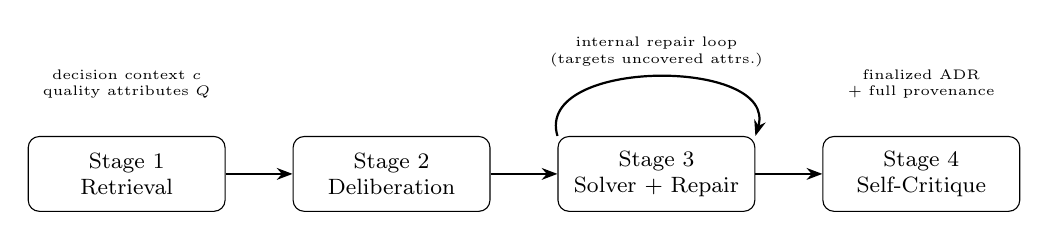
\begin{tikzpicture}[
  stage/.style={draw, rounded corners, minimum width=2.5cm, minimum height=0.95cm, align=center, font=\footnotesize},
  arr/.style={-{Stealth[length=2mm]}, thick},
  node distance=0.85cm
]
\node[stage] (retrieval) {Stage 1\\Retrieval};
\node[stage, right=of retrieval] (delib) {Stage 2\\Deliberation};
\node[stage, right=of delib] (solver) {Stage 3\\Solver + Repair};
\node[stage, right=of solver] (critique) {Stage 4\\Self-Critique};

\draw[arr] (retrieval) -- (delib);
\draw[arr] (delib) -- (solver);
\draw[arr] (solver) -- (critique);

\draw[arr] (solver.north west) .. controls +(-0.3,1.0) and +(0.3,1.0) .. (solver.north east)
  node[midway, above, font=\tiny, align=center] {internal repair loop\\(targets uncovered attrs.)};

\node[above=0.35cm of retrieval, font=\tiny, align=center] {decision context $c$\\quality attributes $Q$};
\node[above=0.35cm of critique, font=\tiny, align=center] {finalized ADR\\+ full provenance};
\end{tikzpicture}
\caption{The CADENCE pipeline. Each stage consumes the previous stage's output; Stage~3's repair loop is internal to Stage~3 --- it never re-enters Stage~2's multi-agent deliberation --- and issues a standalone repair call driven by the solver's uncovered-attribute signal (with the unsatisfiable core reported only as a supplementary diagnostic), iterating to a fixed cap before Stage~4 finalizes the decision.\label{fig:pipeline}}
\end{figure}
\FloatBarrier

\begin{figure}[!htbp]
\centering
\adjustbox{max width=\textwidth}{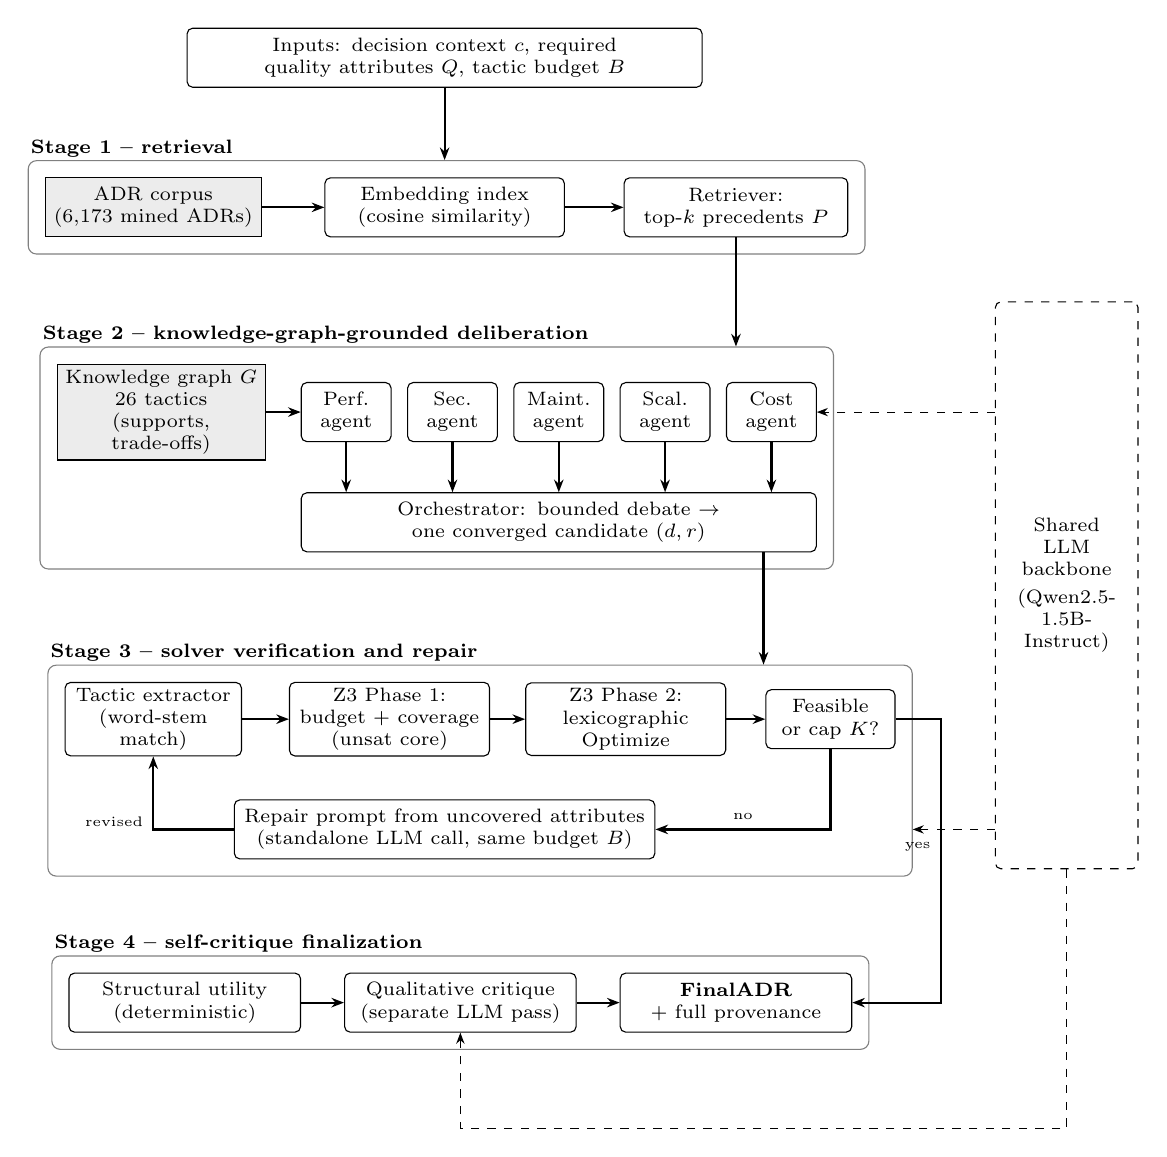
\begin{tikzpicture}[
  font=\scriptsize,
  box/.style={draw, rounded corners=2pt, align=center, minimum height=0.75cm, inner sep=2pt},
  store/.style={draw, align=center, minimum height=0.75cm, inner sep=2pt, fill=gray!15},
  ext/.style={draw, dashed, rounded corners=2pt, align=center, inner sep=3pt},
  layer/.style={draw=gray, rounded corners=3pt, inner xsep=6pt, inner ysep=6pt},
  lbl/.style={font=\scriptsize\bfseries, anchor=south west, inner sep=1pt},
  arr/.style={-{Stealth[length=1.6mm]}, thick},
  darr/.style={-{Stealth[length=1.4mm]}, dashed},
]
% ---- inputs
\node[box, text width=6.4cm] (inp) at (5.2,12.7) {Inputs: decision context $c$, required quality attributes $Q$, tactic budget $B$};

% ---- Stage 1
\node[store, text width=2.6cm] (corpus) at (1.5,10.8) {ADR corpus\\(6{,}173 mined ADRs)};
\node[box, text width=2.9cm] (index) at (5.2,10.8) {Embedding index\\(cosine similarity)};
\node[box, text width=2.7cm] (retr) at (8.9,10.8) {Retriever:\\top-$k$ precedents $P$};
\begin{scope}[on background layer]
\node[layer, fit=(corpus)(index)(retr)] (L1) {};
\end{scope}
\node[lbl] at (L1.north west) {Stage 1 -- retrieval};

% ---- Stage 2
\node[store, text width=2.5cm] (kg) at (1.6,8.2) {Knowledge graph $G$\\26 tactics\\(supports, trade-offs)};
\foreach \x/\n/\t in {3.95/Perf/Perf.,5.3/Sec/Sec.,6.65/Maint/Maint.,8.0/Scal/Scal.,9.35/Cost/Cost}
  \node[box, text width=1.0cm] (ag\n) at (\x,8.2) {\t\\agent};
\node[box, text width=6.4cm] (orch) at (6.65,6.8) {Orchestrator: bounded debate $\rightarrow$ one converged candidate $(d,r)$};
\begin{scope}[on background layer]
\node[layer, fit=(kg)(agPerf)(agCost)(orch)] (L2) {};
\end{scope}
\node[lbl] at (L2.north west) {Stage 2 -- knowledge-graph-grounded deliberation};

% ---- Stage 3
\node[box, text width=2.1cm] (ext) at (1.5,4.3) {Tactic extractor\\(word-stem match)};
\node[box, text width=2.4cm] (z1) at (4.5,4.3) {Z3 Phase 1:\\budget + coverage\\(unsat core)};
\node[box, text width=2.4cm] (z2) at (7.5,4.3) {Z3 Phase 2:\\lexicographic\\Optimize};
\node[box, text width=1.5cm] (dec) at (10.1,4.3) {Feasible\\or cap $K$?};
\node[box, text width=5.2cm] (rep) at (5.2,2.9) {Repair prompt from uncovered attributes\\(standalone LLM call, same budget $B$)};
\begin{scope}[on background layer]
\node[layer, fit=(ext)(z1)(z2)(dec)(rep)] (L3) {};
\end{scope}
\node[lbl] at (L3.north west) {Stage 3 -- solver verification and repair};

% ---- Stage 4
\node[box, text width=2.8cm] (su) at (1.9,0.7) {Structural utility\\(deterministic)};
\node[box, text width=2.8cm] (qc) at (5.4,0.7) {Qualitative critique\\(separate LLM pass)};
\node[box, text width=2.8cm] (fin) at (8.9,0.7) {\textbf{FinalADR}\\+ full provenance};
\begin{scope}[on background layer]
\node[layer, fit=(su)(qc)(fin)] (L4) {};
\end{scope}
\node[lbl] at (L4.north west) {Stage 4 -- self-critique finalization};

% ---- shared LLM backbone
\node[ext, text width=1.6cm, minimum height=7.2cm] (llm) at (13.1,6.0) {Shared\\LLM\\backbone\\[2pt](Qwen2.5-\\1.5B-\\Instruct)};

% ---- main flow
\draw[arr] (inp.south) -- (inp |- L1.north);
\draw[arr] (corpus) -- (index);
\draw[arr] (index) -- (retr);
\draw[arr] (retr.south) -- (retr.south |- L2.north);
\draw[arr] (kg) -- (agPerf);
\foreach \n in {Perf,Sec,Maint,Scal,Cost} \draw[arr] (ag\n.south) -- (ag\n.south |- orch.north);
\draw[arr] ([xshift=2.6cm]orch.south) -- ([xshift=2.6cm]orch.south |- L3.north);
\draw[arr] (ext) -- (z1);
\draw[arr] (z1) -- (z2);
\draw[arr] (z2) -- (dec);
\draw[arr] (dec.south) |- node[pos=0.75,above,font=\tiny]{no} (rep.east);
\draw[arr] (rep.west) -| node[pos=0.55,left,font=\tiny]{revised} (ext.south);
\draw[arr] (dec.east) -- (11.5,4.3) -- node[pos=0.45,left,font=\tiny]{yes} (11.5,0.7) -- (fin.east);
\draw[arr] (su) -- (qc);
\draw[arr] (qc) -- (fin);

% ---- LLM usage (dashed)
\draw[darr] (llm.west |- agCost) -- (agCost.east);
\draw[darr] (llm.west |- rep) -- (L3.east |- rep);
\draw[darr] (llm.south) -- (13.1,-0.9) -- (5.4,-0.9) -- (qc.south);
\end{tikzpicture}
}
\caption{Component architecture of CADENCE. Solid arrows are data flow, dashed arrows are calls to the shared LLM backbone. Stage~1 reads the mined ADR corpus through an embedding index; Stage~2 composes five quality-attribute agents grounded in the tactic knowledge graph~$G$ under one orchestrator; Stage~3 turns the candidate into a Z3 instance and loops through a standalone repair call until the instance is feasible or the repair cap~$K$ is reached; Stage~4 combines a deterministic structural score with a separate LLM critique into the final ADR with full provenance.\label{fig:architecture}}
\end{figure}
\FloatBarrier

\begin{figure}[!htbp]
\centering
\adjustbox{max width=\textwidth}{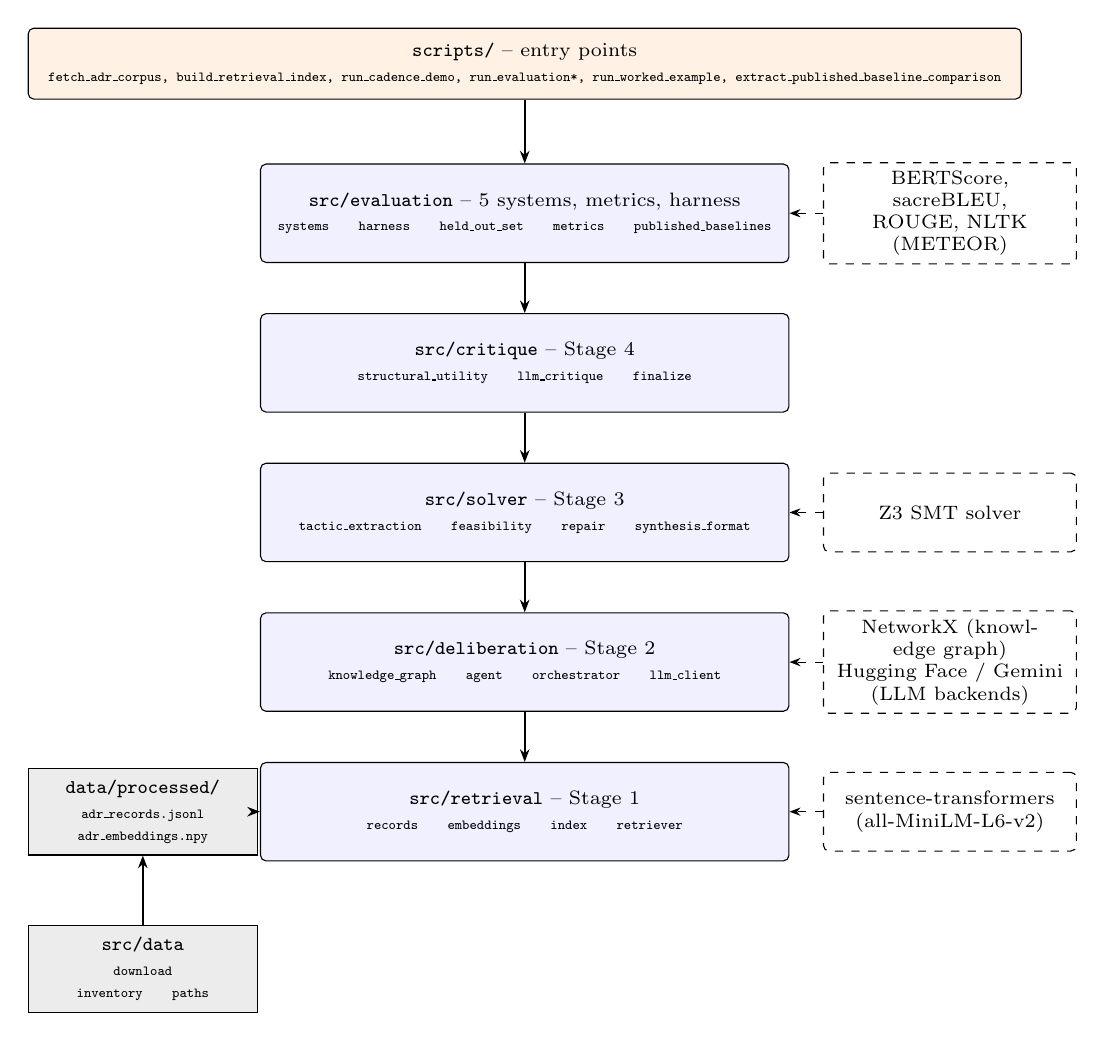
\begin{tikzpicture}[
  font=\scriptsize,
  pkg/.style={draw, rounded corners=2pt, align=center, text width=6.5cm, minimum height=1.25cm, inner sep=3pt, fill=blue!6},
  data/.style={draw, align=center, text width=2.7cm, minimum height=1.1cm, inner sep=3pt, fill=gray!15},
  ext/.style={draw, dashed, rounded corners=2pt, align=center, text width=3.0cm, minimum height=1.0cm, inner sep=3pt},
  top/.style={draw, rounded corners=2pt, align=center, text width=12.4cm, minimum height=0.9cm, inner sep=3pt, fill=orange!10},
  arr/.style={-{Stealth[length=1.6mm]}, thick},
  darr/.style={-{Stealth[length=1.4mm]}, dashed},
]
\node[top] (scripts) at (6.3,10.3) {\textbf{\texttt{scripts/}} -- entry points\\[1pt]{\tiny\ttfamily fetch\_adr\_corpus, build\_retrieval\_index, run\_cadence\_demo, run\_evaluation*, run\_worked\_example, extract\_published\_baseline\_comparison}};

\node[pkg] (ev) at (6.3,8.4) {\textbf{\texttt{src/evaluation}} -- 5 systems, metrics, harness\\[1pt]\modl{systems ~~ harness ~~ held\_out\_set ~~ metrics ~~ published\_baselines}};
\node[pkg] (cr) at (6.3,6.5) {\textbf{\texttt{src/critique}} -- Stage 4\\[1pt]\modl{structural\_utility ~~ llm\_critique ~~ finalize}};
\node[pkg] (so) at (6.3,4.6) {\textbf{\texttt{src/solver}} -- Stage 3\\[1pt]\modl{tactic\_extraction ~~ feasibility ~~ repair ~~ synthesis\_format}};
\node[pkg] (de) at (6.3,2.7) {\textbf{\texttt{src/deliberation}} -- Stage 2\\[1pt]\modl{knowledge\_graph ~~ agent ~~ orchestrator ~~ llm\_client}};
\node[pkg] (re) at (6.3,0.8) {\textbf{\texttt{src/retrieval}} -- Stage 1\\[1pt]\modl{records ~~ embeddings ~~ index ~~ retriever}};

\node[data] (dt) at (1.45,-1.2) {\textbf{\texttt{src/data}}\\[1pt]\modl{download ~~ inventory ~~ paths}};
\node[data] (art) at (1.45,0.8) {\texttt{data/processed/}\\[1pt]\modl{adr\_records.jsonl}\\\modl{adr\_embeddings.npy}};

\node[ext] (e1) at (11.7,0.8) {sentence-transformers\\(all-MiniLM-L6-v2)};
\node[ext] (e2) at (11.7,2.7) {NetworkX (knowledge graph)\\Hugging Face / Gemini\\(LLM backends)};
\node[ext] (e3) at (11.7,4.6) {Z3 SMT solver};
\node[ext] (e4) at (11.7,8.4) {BERTScore, sacreBLEU,\\ROUGE, NLTK (METEOR)};

\draw[arr] (scripts.south -| ev) -- (ev.north);
\draw[arr] (ev) -- (cr);
\draw[arr] (cr) -- (so);
\draw[arr] (so) -- (de);
\draw[arr] (de) -- (re);
\draw[arr] (dt) -- (art);
\draw[arr] (art) -- (re);
\draw[darr] (e1) -- (re);
\draw[darr] (e2) -- (de);
\draw[darr] (e3) -- (so);
\draw[darr] (e4) -- (ev);
\end{tikzpicture}
}
\caption{Software architecture of the released implementation, as a stack of Python packages. Solid arrows are import dependencies between adjacent layers (no package imports from a package above it); dashed arrows are third-party libraries. Packages \texttt{src/retrieval}, \texttt{src/deliberation}, \texttt{src/solver} and \texttt{src/critique} correspond to Stages~1--4; \texttt{src/evaluation} reimplements the four baselines and computes the metrics; \texttt{src/data} fetches and inventories the corpus that \texttt{src/retrieval} parses.\label{fig:implementation}}
\end{figure}
\FloatBarrier

\begin{algorithm}[t]
\caption{CADENCE}
\label{alg:cadence}
\begin{algorithmic}[1]
\REQUIRE context $c$, quality attributes $Q$, tactic budget $B$, tactic catalog with graph $G$, max deliberation rounds $R$, max repair iterations $K$
\ENSURE finalized decision with provenance
\STATE $P \gets \textsc{Retrieve}(c)$ \COMMENT{Stage 1: top-$k$ precedents}
\STATE $(d, r) \gets \textsc{Deliberate}(c, P, Q, G, R)$ \COMMENT{Stage 2: bounded multi-agent debate}
\STATE $i \gets 0$; $\mathit{best} \gets \bot$
\LOOP
  \STATE $\mathit{res} \gets \textsc{CheckFeasibility}(d, Q, B, G)$ \COMMENT{Stage 3, Phase 1+2}
  \IF{$\mathit{best} = \bot$ \textbf{or} $|\mathit{res}.\mathit{covered}| > |\mathit{best}.\mathit{res}.\mathit{covered}|$}
    \STATE $\mathit{best} \gets (\mathit{res}, d, r)$ \COMMENT{track highest-coverage attempt seen so far}
  \ENDIF
  \IF{$\mathit{res}.\mathit{feasible}$ \textbf{or} $i = K$}
    \STATE \textbf{break} \COMMENT{degrade gracefully with a caveat if infeasible}
  \ENDIF
  \STATE $(d, r) \gets \textsc{Repair}(d, \mathit{res}.\mathit{uncovered}, B)$ \COMMENT{standalone LLM repair call, targets uncovered attributes}
  \STATE $i \gets i + 1$
\ENDLOOP
\STATE $(\mathit{res}, d, r) \gets \mathit{best}$ \COMMENT{use the best attempt seen, not necessarily the last}
\STATE $u \gets \textsc{StructuralUtility}(\mathit{res}, G)$ \COMMENT{Stage 4, deterministic}
\STATE $q \gets \textsc{QualitativeCritique}(d, r, Q)$ \COMMENT{Stage 4, separate LLM pass}
\RETURN $\textsc{Finalize}(d, r, u, q, \mathit{res}, P)$
\end{algorithmic}
\end{algorithm}

\subsection{Stage 1: Retrieval-Augmented Case-Based Reasoning}

Stage 1 embeds the decision context $c$ with a sentence-embedding model and retrieves the $k$ nearest precedent ADRs, by cosine similarity, from a dense vector index built over the full corpus of $6{,}173$ real, mined ADRs (Section~\ref{sec:evaluation}). Each corpus record is parsed leniently from its source Markdown file --- real-world ADR filenames and internal structure are inconsistent across repositories, so the parser extracts only a title and the full raw body text rather than assuming a fixed section schema. Retrieval returns the top-$k$ precedent records, whose titles are passed into Stage~2 as grounding context; when used inside a held-out evaluation, the query record's own ground-truth ADR is excluded from its own retrieval results to prevent leakage.

\subsection{Stage 2: Knowledge-Graph-Grounded Multi-Agent Deliberation}

Stage 2 instantiates one \texttt{QualityAttributeAgent} per required quality attribute in $Q$. Each agent is grounded in a knowledge graph $G$ built from a hand-curated catalog of 26 architectural tactics spanning the five quality attributes (5 or 6 per attribute; Table~\ref{tab:tactics} lists the full catalog), where each tactic node has a directed \emph{supports} edge to the quality attribute it primarily serves and directed \emph{trade-off} edges, annotated with a natural-language explanation, to every other attribute it is known to burden --- for instance, \emph{caching} supports \emph{performance} but trades off against \emph{maintainability} via cache-invalidation complexity, and \emph{authentication} supports \emph{security} but trades off against both \emph{performance} (verification latency) and \emph{cost\_operability} (identity-infrastructure upkeep), as Figure~\ref{fig:kg-excerpt} depicts. Given the decision context and Stage~1's retrieved precedents, each agent proposes a candidate decision serving its own attribute using $G$'s \emph{supports} edges, and may critique candidates proposed by other agents; $G$'s \emph{trade-off} edges are consumed downstream by Stage~3's feasibility optimization and Stage~4's utility score, rather than injected into Stage~2's prompts. Deliberation proceeds for a bounded number of rounds (\texttt{max\_rounds}), after which an orchestrator synthesizes the debate into one converged candidate decision and rationale.

\begin{figure}[!htbp]
\centering
\resizebox{\columnwidth}{!}{%
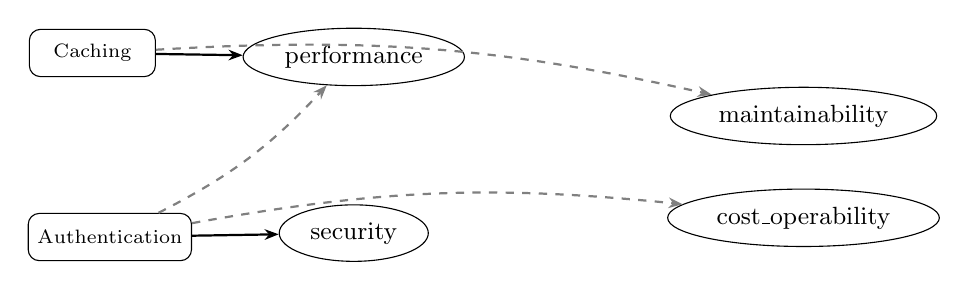
\begin{tikzpicture}[
  qa/.style={draw, ellipse, minimum width=1.55cm, minimum height=0.7cm, align=center, font=\small},
  tac/.style={draw, rounded corners, minimum width=1.6cm, minimum height=0.6cm, align=center, font=\scriptsize},
  supp/.style={-{Stealth[length=1.8mm]}, thick},
  trad/.style={-{Stealth[length=1.8mm]}, dashed, thick, gray},
  node distance=0.55cm and 1.15cm
]
\node[qa] (perf) {performance};
\node[qa, below=1.5cm of perf] (sec) {security};
\node[qa, right=2.6cm of perf, yshift=-0.75cm] (maint) {maintainability};
\node[qa, below=0.55cm of maint] (cost) {cost\_\allowbreak operability};
\node[tac, left=1.1cm of perf, yshift=0.05cm] (caching) {Caching};
\node[tac, left=1.1cm of sec, yshift=-0.05cm] (auth) {Authentication};

\draw[supp] (caching) -- (perf);
\draw[trad] (caching) to[bend left=8] (maint);
\draw[supp] (auth) -- (sec);
\draw[trad] (auth) to[bend right=10] (perf);
\draw[trad] (auth) to[bend left=8] (cost);
\end{tikzpicture}%
}
\caption{Excerpt of knowledge graph $G$: solid arrows are \emph{supports} edges, dashed gray arrows are \emph{trade-off} edges. Only 2 of the catalog's 26 tactics and 4 of its 5 quality attributes are shown for legibility.\label{fig:kg-excerpt}}
\end{figure}
\FloatBarrier

\begin{table}[!htbp]
\caption{The 26-Tactic Catalog Grounding Stage 2's Knowledge Graph $G$. The number in parentheses is the count of \emph{trade-off} edges the tactic carries to other quality attributes (0--2 in this catalog); each tactic's \emph{supports} edge targets the quality attribute in its row.\label{tab:tactics}}
\centering
\footnotesize
\setlength{\tabcolsep}{4pt}
\begin{tabular}{@{}>{\raggedright\arraybackslash}p{0.95in}>{\raggedright\arraybackslash}p{4.25in}@{}}
\toprule
Quality attribute & Tactics (trade-off edges) \\
\midrule
Performance & Caching (1); connection pooling (1); asynchronous processing via message queues (2); data denormalization (1); read-through/write-behind access (1) \\
Security & Authentication (2); fine-grained authorization (1); encryption in transit/at rest (2); rate limiting/throttling (1); least-privilege service boundaries (1); input validation at trust boundaries (1) \\
Maintainability & Modular decomposition by capability (2); versioned API contracts (1); automated regression test suite (1); centralized structured logging (2); dependency injection/IoC (1) \\
Scalability & Horizontal scaling with stateless instances (2); database sharding (2); event-driven architecture (2); auto-scaling infrastructure (1); read replicas (1) \\
Cost/operability & Managed cloud services (2); infrastructure as code (0); multi-tenancy (2); serverless/FaaS deployment (2); circuit breaker for dependencies (1) \\
\bottomrule
\end{tabular}

\vspace{2pt}
\footnotesize Per-tactic effects, trade-off targets, and the natural-language rationale for each edge are in \texttt{src/deliberation/knowledge\_graph.py} (see Data and Code Availability).
\end{table}
\FloatBarrier

Synthesis is the stage's most format-fragile step: it asks the underlying LLM to emit a structured \texttt{CANDIDATE}/\texttt{RATIONALE} response that Stage~3 can parse deterministically. In practice, real small-model output deviates from any single expected format in ways a fixed parser cannot fully anticipate in advance (Section~\ref{sec:method-robustness}); the orchestrator therefore retries the same synthesis prompt up to three times on a parse failure before surfacing an error, since generation is stochastic and a differently-sampled retry frequently self-corrects a formatting slip that a hand-written regex extension would not have anticipated.

\subsection{Stage 3: Constraint-Solver-Verified Feasibility with Repair Loop}
\label{sec:method-stage3}

Stage 2's converged candidate is free text: a human-readable decision and rationale, not a structured commitment a solver can reason about directly. Stage 3 first extracts which of the 26 catalog tactics the candidate text actually mentions, via fuzzy word-stem overlap against each tactic's name, giving Boolean decision variables $\{t_1, \ldots, t_m\}$, one per mentioned tactic. It then checks feasibility in two phases against the Z3 SMT solver.

\emph{Phase 1 (strict feasibility).} A budget constraint $\sum_i t_i \leq B$ (a caller-specified tactic budget $B$) and, for every required quality attribute $q \in Q$, a coverage constraint $\bigvee_{i \,:\, \mathrm{supports}(t_i) = q} t_i$ (at least one selected tactic must support $q$) are asserted with \texttt{assert\_and\_track}, so that if the instance is unsatisfiable, Z3 returns an \emph{unsatisfiable core}: the constraints jointly responsible for infeasibility. This core is a useful, but not necessarily complete, diagnostic --- Z3's core-extraction semantics can name only one of several symmetric zero-coverage attributes as blocking, omitting others equally unsatisfied --- so Stage~3 does not treat it as authoritative.

\emph{Phase 2 (best-effort optimized selection).} A separate \texttt{Optimize} instance re-asserts the budget constraint and searches for the tactic selection that jointly (a) maximizes how many required quality attributes are covered and (b) minimizes the caller-weighted cost of the trade-offs incurred, always returning a concrete selection even when Phase~1 found the instance strictly infeasible. These two objectives are declared under Z3's \texttt{priority="lex"} lexicographic mode as separate \texttt{add\_soft} groups, rather than one weighted-sum objective --- a distinction we verified matters empirically. An earlier weighted-sum formulation used a single large constant to bias coverage above trade-off cost, but because trade-off weights are caller-supplied with no upper bound, a selection accumulating enough trade-off weight could mathematically outvote a required attribute's coverage regardless of the bias constant's size (a concrete repro during development: four trade-offs at weight 300 each outweighed a coverage bias of 1000). Lexicographic priority makes coverage strictly dominate trade-off avoidance independent of weight magnitude --- the only encoding safe for caller-supplied weights whose scale cannot be bounded in advance. The resulting \texttt{covered\_quality\_attributes} / \texttt{uncovered\_quality\_attributes} split from this phase, not Phase~1's unsat core, is the sound and complete signal of what still needs fixing.

If Phase~1 finds the instance infeasible, Stage~3 constructs a repair prompt naming, for every uncovered attribute, the concrete tactics that would cover it, and asks the LLM to revise the candidate within the same budget. This is re-checked against the solver, iterating up to \texttt{max\_repair\_iterations} times and tracking the best (highest-coverage) attempt seen. If the budget is never satisfiable within the cap, Stage~3 returns the best attempt found with an explicit caveat rather than silently accepting an infeasible decision or discarding an otherwise-reasonable candidate; a transient LLM or parse failure during any repair attempt triggers the next iteration, not an abort.

\subsection{Stage 4: Self-Critique Finalization}
\label{sec:method-stage4}

Stage 4 combines two independently-computed signals into each quality attribute's final utility score. The \emph{structural} component is deterministic: for attribute $q$, it is $1.0$ if $q$ is among the solver-verified decision's covered attributes, minus a fixed penalty of $0.2$ for every incoming trade-off edge from a selected tactic onto $q$ in $G$, floored at $0.0$; it depends only on Stage~3's already-verified output and involves no further LLM call. The \emph{qualitative} component is a single LLM pass scoring every required attribute on a 0--10 scale and flagging any residual weakness, given the full decision, rationale, and attribute list in one call; parsing uses a three-tier matcher --- a strict same-line pattern, a tolerant same-line fallback, and a heading-section fallback for responses that state an attribute as its own heading with the field on a separate, unlabeled line (Section~\ref{sec:method-robustness}) --- so a loose regex cannot lock onto a prose preamble instead of the real scored line, and the call is retried up to three times on a parse failure as Stage~2's synthesis call is. The two components combine as $\mathrm{combined}_q = 0.5 \cdot \mathrm{structural}_q \cdot 10 + 0.5 \cdot \mathrm{qualitative}_q$, and overall decision utility is the mean combined score across all required attributes. The finalized \texttt{FinalADR} carries this scoring together with full provenance --- retrieved precedents, the complete per-agent deliberation transcript, which tactics were selected and by which repair iteration, and any solver caveat --- so the decision is auditable end-to-end.

\subsection{Implementation Robustness: Parsing Real, Stochastic LLM Output}
\label{sec:method-robustness}

A structured-output prompt's hand-written happy-path parser reliably breaks against a real, deployed small language model, and our development process surfaced this repeatedly and concretely, not as a theoretical concern. Running the full pipeline end-to-end against Qwen2.5-1.5B-Instruct, the reproducible local backbone used throughout this work, produced six distinct real formatting deviations across Stages~2--4, summarized in Table~\ref{tab:deviations}.

\begin{table}[!htbp]
\caption{Six Real LLM Output-Format Deviations Encountered\label{tab:deviations}}
\centering
\footnotesize
\setlength{\tabcolsep}{3pt}
\begin{tabular}{@{}
  >{\centering\arraybackslash}p{0.15in}
  >{\raggedright\arraybackslash}p{1.55in}
  >{\raggedright\arraybackslash}p{1.65in}
@{}}
\toprule
\# & Deviation & Resolved by \\
\midrule
1 & Extra descriptor word (``Candidate Decision:'' for ``Candidate:'') & Tolerant same-line parser \\
2 & Non-literal ``no weakness'' (``None identified'' for literal ``none'') & Tolerant same-line parser \\
3 & Fraction-style score (``8/10''), this model's \emph{default} 0--10 answer & Tolerant same-line parser \\
4 & Prose preamble a loose regex could lock onto instead of the real line & Tolerant same-line parser \\
5 & Genuine word substitution (``Candidacy:'' for ``Candidate:''), unanticipatable by regex tolerance & Bounded retry (2--3 attempts) \\
6 & Attribute-as-heading structure: attribute on its own heading line, field unlabeled on a later line & Third parser tier (heading-section fallback) \\
\bottomrule
\end{tabular}
\end{table}
\FloatBarrier

The first four are addressable by a sufficiently tolerant same-line parser. The fifth is not, and its discovery motivated this work's general strategy of pairing every structured-output prompt with a bounded retry (two to three attempts) of the identical prompt on a parse failure, rather than special-casing wording variants indefinitely; because generation is stochastic, a differently-sampled retry frequently self-corrects a slip the parser did not anticipate, and Stages~2, 3, and 4 all apply this pattern. The sixth, discovered later during the scaled evaluation run (e.g.\ \texttt{**Performance**} followed, several lines later, by \texttt{**Score:** 9/10} with no attribute name on that line), shows retry's limit: it exhausted all three attempts because it was not a stochastic one-off but a genuinely different \emph{structure} no same-line pattern, however tolerant, could match --- fixing it required a third parser tier (Section~\ref{sec:method-stage4}) that locates an attribute's heading and searches only the bounded section up to the next heading for an unlabeled field. We report this as a methodological finding in its own right: any system asking an LLM for structured intermediate output a downstream deterministic component must consume should validate its parser against real, repeated model output before trusting it unattended, treat bounded retry as the general-purpose fix for wording variation, and expect that a genuinely new structural format will eventually require a genuinely new parser tier --- discoverable only by actually running the real pipeline.

\subsection{Worked Example}
\label{sec:worked-example}

To make the four stages concrete, this section walks through one real, complete run of the pipeline reported verbatim from the actual implementation (\texttt{scripts/run\_worked\_example.py}) --- illustrative, not an evaluation data point; this paper's quantitative claims come from Section~\ref{sec:evaluation}'s held-out runs, not this example.

Given a context describing a 10x read-traffic surge on an order-processing service, with requirements to keep p99 latency low, stay operable by a small team, and avoid new security risk, \textbf{Stage 1} retrieves three real precedents on message brokering, server architecture, and JWT inter-service authentication. \textbf{Stage 2} runs two rounds across the five agents: the \emph{performance} agent proposes a message queue to decouple reads from the application server; the \emph{security} agent independently argues for JWT authentication, encryption, and rate limiting; the \emph{cost\_operability} agent's round-2 critique flags a real cross-attribute tension, that the message broker's added network overhead ``could affect real-time interactions.'' The orchestrator synthesizes these into one converged candidate, from which Stage~3 extracts a tactic selection.

\textbf{Stage 3} extracts three catalog tactics --- \emph{asynchronous processing via message queues}, \emph{event-driven architecture}, and \emph{serverless/FaaS deployment} --- covering \emph{performance}, \emph{scalability}, and \emph{cost\_operability}, but not \emph{maintainability} or \emph{security}. This example runs at $B=4$, which, as Section~\ref{sec:evaluation} establishes, cannot cover all five attributes under a catalog where each tactic supports exactly one --- unlike the scaled run's $B=5$ condition, it is not a test of achievable-budget feasibility. It nonetheless illustrates the repair loop's mechanics: one tactic slot remained within budget, but the candidate's text never named a fourth, security- or maintainability-covering tactic for the extractor to find. Both repair attempts fail to close the gap, and Stage~3 returns the best-effort selection with an explicit caveat naming the covered and unaddressed attributes.

\textbf{Stage 4} finalizes the decision --- a microservices architecture using a message queue, an event-sourcing database, and serverless functions --- and scores it per attribute (Table~\ref{tab:worked-example}; Figure~\ref{fig:example-architecture} draws the resulting architecture), flagging a concrete weakness for each (e.g., for \emph{security}: serverless functions carry function-timeout limits and reduced control over the execution environment). The two uncovered attributes' structural components are correctly $0.0$, dragging their combined scores down even where the qualitative pass alone would have scored the prose favorably --- exactly the blending Section~\ref{sec:method-stage4} argues for.

\begin{table}[!htbp]
\caption{Worked Example (Illustrative, $B=4$, Not an Evaluation Data Point): Per-Attribute Utility Scores (Overall: 6.6/10)\label{tab:worked-example}}
\centering
\footnotesize
\begin{adjustbox}{max width=\textwidth}
\begin{tabular}{@{}lccc@{}}
\toprule
Quality Attribute & Structural & Qualitative & Combined \\
\midrule
Performance       & 0.8 & 8.0 & 8.0 \\
Security          & 0.0 & 9.0 & 4.5 \\
Maintainability   & 0.0 & 7.0 & 3.5 \\
Scalability       & 1.0 & 8.0 & 9.0 \\
Cost/Operability  & 1.0 & 6.0 & 8.0 \\
\bottomrule
\end{tabular}
\end{adjustbox}
\end{table}
\FloatBarrier

\begin{figure}[!htbp]
\centering
\adjustbox{max width=\textwidth}{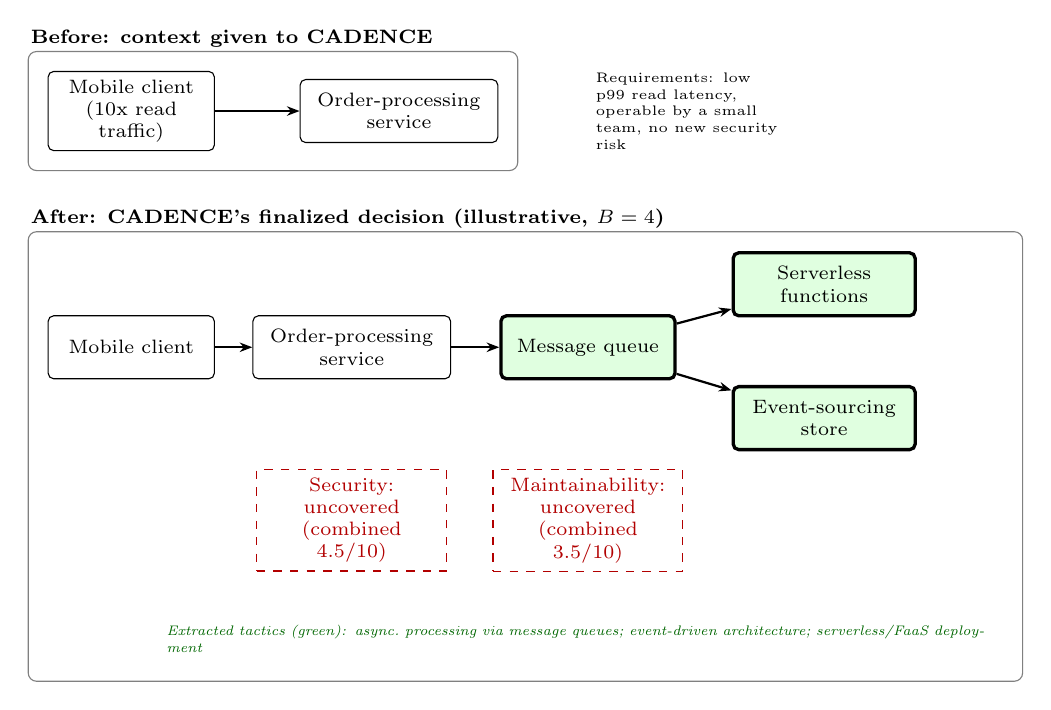
\begin{tikzpicture}[
  font=\scriptsize,
  comp/.style={draw, rounded corners=2pt, align=center, minimum height=0.8cm, inner sep=3pt},
  new/.style={draw, rounded corners=2pt, align=center, minimum height=0.8cm, inner sep=3pt, fill=green!12, very thick},
  gap/.style={draw, dashed, red!70!black, align=center, minimum height=0.8cm, inner sep=3pt, text=red!70!black},
  panel/.style={draw=gray, rounded corners=3pt, inner sep=7pt},
  lbl/.style={font=\scriptsize\bfseries, anchor=south west, inner sep=1pt},
  arr/.style={-{Stealth[length=1.6mm]}, thick},
  tac/.style={font=\tiny\itshape, align=center, text=green!40!black},
]
% ---- before
\node[comp, text width=1.9cm] (mc0) at (1.2,5.2) {Mobile client\\(10x read traffic)};
\node[comp, text width=2.3cm] (os0) at (4.6,5.2) {Order-processing\\service};
\draw[arr] (mc0) -- (os0);
\begin{scope}[on background layer]
\node[panel, fit=(mc0)(os0)] (P0) {};
\end{scope}
\node[lbl] at (P0.north west) {Before: context given to CADENCE};
\node[font=\tiny, align=left, text width=2.4cm] at (8.3,5.2) {Requirements: low p99 read latency, operable by a small team, no new security risk};

% ---- after
\node[comp, text width=1.9cm] (mc) at (1.2,2.2) {Mobile client};
\node[comp, text width=2.3cm] (os) at (4.0,2.2) {Order-processing\\service};
\node[new, text width=2.0cm] (mq) at (7.0,2.2) {Message queue};
\node[new, text width=2.1cm] (fn) at (10.0,3.0) {Serverless\\functions};
\node[new, text width=2.1cm] (es) at (10.0,1.3) {Event-sourcing\\store};
\draw[arr] (mc) -- (os);
\draw[arr] (os) -- (mq);
\draw[arr] (mq) -- (fn);
\draw[arr] (mq) -- (es);
\node[gap, text width=2.2cm] (g1) at (4.0,0.0) {Security: uncovered\\(combined 4.5/10)};
\node[gap, text width=2.2cm] (g2) at (7.0,0.0) {Maintainability: uncovered\\(combined 3.5/10)};
\node[font=\tiny\itshape, text width=10.5cm, align=left, text=green!40!black] (leg) at (6.9,-1.5) {Extracted tactics (green): async.\ processing via message queues; event-driven architecture; serverless/FaaS deployment};
\begin{scope}[on background layer]
\node[panel, fit=(mc)(os)(mq)(fn)(es)(g1)(g2)(leg)] (P1) {};
\end{scope}
\node[lbl] at (P1.north west) {After: CADENCE's finalized decision (illustrative, $B=4$)};
\end{tikzpicture}
}
\caption{The worked example as an architecture. Top: the context given to CADENCE. Bottom: the components named in the finalized decision (green: tactics the extractor found) and the two quality attributes the decision leaves uncovered (red, with their combined utility scores from Table~\ref{tab:worked-example}). The topology is schematic: the run reports which components were selected, not how they are wired.\label{fig:example-architecture}}
\end{figure}
\FloatBarrier

\section{Evaluation}
\label{sec:evaluation}

\subsection{Corpus and Experimental Setup}

We evaluate against the ``Context Matters'' replication package~\citep{contextmatters-zenodo} (Zenodo, DOI:~10.5281/zenodo.18370195), derived from the same mining study that provides Stage~1's retrieval corpus~\citep{buchgeher2023adr}. The package's own \texttt{dataset\_index.json} catalogs 954 repository folders with an extraction-confidence status each (750 \texttt{Verified}, 96 \texttt{Doubt (name sequence)}, 40 \texttt{Repo Inaccessible}, 33 \texttt{Doubt (no repo dir)}, 30 \texttt{Doubt (missing file)}, 5 \texttt{Doubt (file contents)}); after parsing, the 882 folders with at least one accessible Markdown file yield 6{,}173 individual ADR files (median 4, mean 7.00, maximum 129 per repository, confirming the corpus's documented per-repository sparsity) --- the remaining 72 catalogued folders have no accessible file and contribute nothing to either count, drawn almost, but not entirely, along status lines (39 of 40 \texttt{Repo Inaccessible}, 32 of 33 \texttt{Doubt (no repo dir)}, 1 of 5 \texttt{Doubt (file contents)}; every folder under the remaining two statuses contributes at least one file). We restrict our held-out evaluation set to the 750 folders marked \texttt{Verified}, so ground-truth quality is not itself a confound. Following this corpus's own upstream precedent (its companion sub-study is titled ``ADR Generation from Titles''), we construct each held-out query as the record's title and treat its full body as ground truth, matching the task formulation the retrieval-only baseline is drawn from.

The retrieval index embeds all 6{,}173 records with a sentence-embedding model (\texttt{all-MiniLM-L6-v2}) into a cosine-similarity nearest-neighbor index; a held-out query record is always excluded from its own retrieval results. The local, reproducible LLM backbone used for deliberation, repair, and critique throughout is Qwen2.5-1.5B-Instruct, run via direct \texttt{AutoModelForCausalLM.generate()} calls under CUDA. We disclose deliberation's run-time parameters because they materially affect how Table~\ref{tab:pilot} and Table~\ref{tab:scaled} should be read: the pilot run used $k=2$ and \texttt{max\_rounds=1} (every agent's propose round executed but no agent critiqued another's candidate); the scaled run used $k=3$ and \texttt{max\_rounds=2} (one full critique round). Both runs used \texttt{max\_repair\_iterations=2}, this work's full design default. Table~\ref{tab:pilot}'s \texttt{multiagent\_no\_solver} and \texttt{cadence\_full} columns therefore reflect propose-only deliberation, not adversarial debate; Table~\ref{tab:scaled} does not have this limitation.

\subsection{Baselines and Ablation}

We compare CADENCE (\texttt{cadence\_full}) against four systems forming an ablation ladder that isolates retrieval's, deliberation's, solver verification's, and self-critique's contributions individually --- each step adds exactly one stage over the previous one:

\begin{itemize}[leftmargin=*,itemsep=1pt,topsep=2pt,parsep=0pt]
\item \textbf{Zero-shot} (\texttt{zero\_shot}): a single LLM call given only the decision context, with no retrieval, deliberation, or verification --- the Dhar-et-al.-style baseline~\citep{dhar2024llm}.
\item \textbf{Retrieval-only} (\texttt{retrieval\_only}): the decision context plus Stage~1's top-$k$ retrieved precedent titles, with no deliberation or verification --- the Context-Matters-style baseline~\citep{contextmatters2026}.
\item \textbf{Multi-agent, no solver} (\texttt{multiagent\_no\_solver}): Stages~1--2 in full (retrieval and quality-attribute deliberation), but without Stage~3's solver verification or Stage~4's critique --- the system most structurally comparable to MAAD's~\citep{maad2025} multi-agent premise without its functional-role/LLM-judge design.
\item \textbf{CADENCE, no critique} (\texttt{cadence\_no\_critique}): Stages~1--3 (adds Stage~3's solver-verified feasibility and repair loop over \texttt{multiagent\_no\_solver}), but without Stage~4's self-critique finalization --- isolates solver verification's marginal contribution, and, compared against \texttt{cadence\_full}, self-critique's.
\end{itemize}
Every retrieval-using system routes through the same leakage guard, so no system ever retrieves or is scored against its own query record.

\subsection{Metrics}

We report the four standard generation-quality metrics used in the corpus's own upstream evaluation work, for direct comparability: BERTScore F1, sentence-level BLEU (0--100 scale, via \texttt{sacrebleu}), ROUGE-1 F1, and METEOR, each computed against the held-out record's real, human-authored body text. In addition, only reportable by a solver-verified system, we report \emph{constraint-satisfaction rate} (the fraction of held-out items where Stage~3 reached \texttt{is\_feasible=True}) and \emph{average repair iterations}.

\subsection{Results}

\begin{table}[!htbp]
\caption{Pilot Verification Run ($N=3$, \texttt{tactic\_budget=4}, All 5 Quality Attributes Required --- $B=4$ is mathematically infeasible by construction under this catalog, so \texttt{cadence\_full}'s 0\% constraint-satisfaction rate here is a construction check, not a test of achievable feasibility; see Section~\ref{sec:evaluation})\label{tab:pilot}}
\centering
\begin{adjustbox}{max width=\textwidth}
\begin{tabular}{@{}lcccc@{}}
\toprule
System & BERTScore F1 & BLEU & ROUGE-1 F1 & METEOR \\
\midrule
\texttt{zero\_shot}            & 0.810 & 1.05 & 0.220 & 0.244 \\
\texttt{retrieval\_only}       & 0.819 & 1.71 & 0.216 & 0.250 \\
\texttt{multiagent\_no\_solver}& 0.805 & 1.57 & 0.143 & 0.111 \\
\texttt{cadence\_full}         & 0.801 & 0.59 & 0.138 & 0.102 \\
\bottomrule
\end{tabular}
\end{adjustbox}

\vspace{2pt}
\footnotesize \texttt{cadence\_full}: constraint-satisfaction rate 0.00, average repair iterations 2.00 (see discussion below).
\end{table}
\FloatBarrier

Table~\ref{tab:pilot} reports a small-$N$ pilot run used to verify the full pipeline and evaluation harness end-to-end before committing to a larger run; we retain it here as a sanity-checked, fully real data point. Table~\ref{tab:scaled} reports our scaled evaluation run: a separate, independent held-out sample ($N=3$, disjoint from the pilot run above) scored under two \texttt{tactic\_budget} conditions --- an achievable budget ($B=5$, matching the number of required quality attributes) and a second, tighter one ($B=2$, included as a construction check on Stage~3's infeasibility handling rather than as a second independent test of achievable feasibility --- see the discussion immediately below) --- with the three budget-independent baselines run once and shared across both conditions (they do not take a \texttt{tactic\_budget} argument). Real end-to-end wall-clock cost per local-model call constrained this scaled run to $N=3$ rather than a larger sample within the time available for this submission; both runs used the same reproducible local backbone described above, and we report the result below as obtained, rather than a larger or cherry-picked sample we did not have time to run.

\begin{table}[!htbp]
\caption{Scaled Evaluation Run ($N=3$, Two \texttt{tactic\_budget} Conditions, Full 5-System Ablation Ladder --- only $B=5$ is arithmetically achievable under this catalog; $B=2$ is mathematically infeasible by construction and reported as a construction check on Stage~3's infeasibility handling, not a second feasibility test; see Section~\ref{sec:evaluation})\label{tab:scaled}}
\centering
\begin{adjustbox}{max width=\textwidth}
\begin{tabular}{@{}lccccc@{}}
\toprule
System & $B$ & BERTScore F1 & BLEU & ROUGE-1 F1 & METEOR \\
\midrule
\texttt{zero\_shot}             & --- & 0.824 & 4.24 & 0.300 & 0.252 \\
\texttt{retrieval\_only}        & --- & 0.813 & 3.76 & 0.312 & 0.238 \\
\texttt{multiagent\_no\_solver} & --- & 0.812 & 0.43 & 0.179 & 0.091 \\
\texttt{cadence\_no\_critique}  & 5   & 0.797 & 0.44 & 0.174 & 0.092 \\
\texttt{cadence\_full}          & 5   & 0.806 & 1.04 & 0.198 & 0.100 \\
\texttt{cadence\_no\_critique}  & 2   & 0.805 & 0.43 & 0.174 & 0.087 \\
\texttt{cadence\_full}          & 2   & 0.802 & 1.57 & 0.186 & 0.104 \\
\bottomrule
\end{tabular}
\end{adjustbox}

\vspace{2pt}
\footnotesize \texttt{cadence\_no\_critique} and \texttt{cadence\_full} at both $B=5$ and $B=2$: constraint-satisfaction rate 0.00, average repair iterations 2.00 (the full \texttt{max\_repair\_iterations=2} design default --- see discussion below for why this run supersedes an earlier one that used \texttt{max\_repair\_iterations=1}).
\end{table}
\FloatBarrier

\begin{figure}[!htbp]
\centering
\adjustbox{max width=\textwidth}{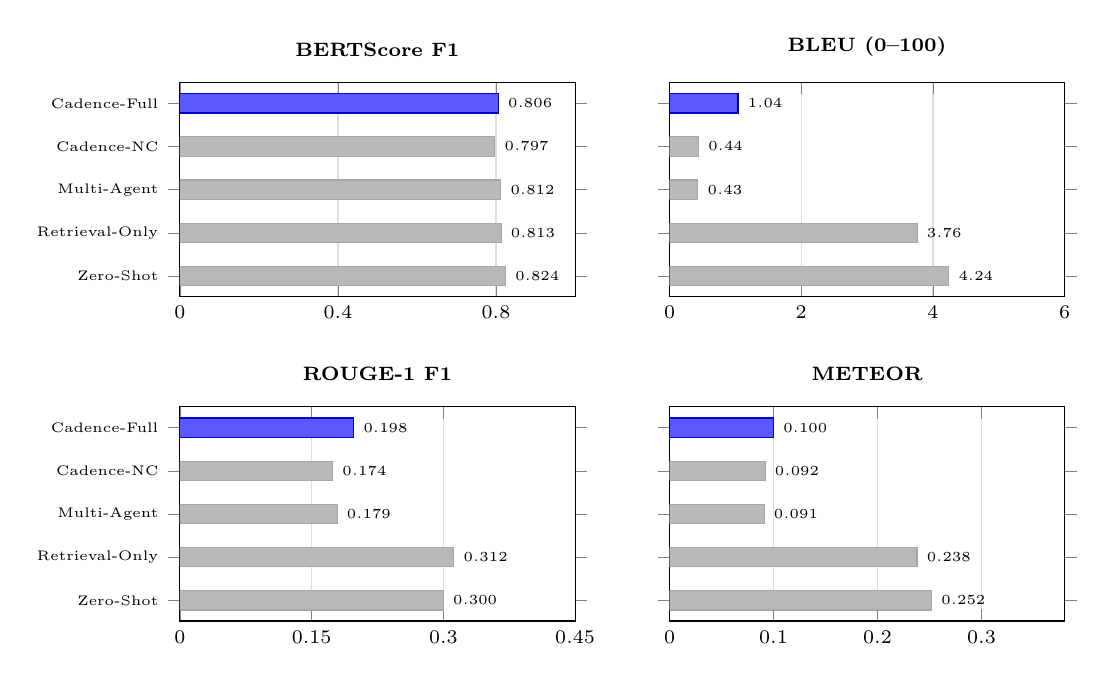
\begin{tikzpicture}
\pgfplotsset{every axis/.append style={
  width=6.6cm, height=4.3cm, xbar, bar width=7pt, xmin=0, enlarge y limits=0.12,
  symbolic y coords={Cadence-Full, Cadence-NC, Multi-Agent, Retrieval-Only, Zero-Shot},
  ytick={Cadence-Full,Cadence-NC,Multi-Agent,Retrieval-Only,Zero-Shot}, y dir=reverse, font=\scriptsize, y tick label style={font=\tiny},
  nodes near coords, nodes near coords align={horizontal}, every node near coord/.append style={font=\tiny, /pgf/number format/fixed, /pgf/number format/fixed zerofill},
  title style={font=\scriptsize\bfseries}, xmajorgrids, grid style={gray!25}}}
\begin{groupplot}[group style={group size=2 by 2, horizontal sep=1.2cm, vertical sep=1.4cm, yticklabels at=edge left}]
\nextgroupplot[title={BERTScore F1}, xmax=1.0, xtick={0,0.4,0.8}, /pgf/number format/precision=3]
\addplot[fill=gray!55, draw=gray!70, bar shift=0pt] coordinates {(0.824,Zero-Shot) (0.813,Retrieval-Only) (0.812,Multi-Agent) (0.797,Cadence-NC)};
\addplot[fill=blue!65, draw=blue!80!black, bar shift=0pt] coordinates {(0.806,Cadence-Full)};
\nextgroupplot[title={BLEU (0--100)}, xmax=6, xtick={0,2,4,6}, /pgf/number format/precision=2]
\addplot[fill=gray!55, draw=gray!70, bar shift=0pt] coordinates {(4.24,Zero-Shot) (3.76,Retrieval-Only) (0.43,Multi-Agent) (0.44,Cadence-NC)};
\addplot[fill=blue!65, draw=blue!80!black, bar shift=0pt] coordinates {(1.04,Cadence-Full)};
\nextgroupplot[title={ROUGE-1 F1}, xmax=0.45, xtick={0,0.15,0.3,0.45}, /pgf/number format/precision=3]
\addplot[fill=gray!55, draw=gray!70, bar shift=0pt] coordinates {(0.300,Zero-Shot) (0.312,Retrieval-Only) (0.179,Multi-Agent) (0.174,Cadence-NC)};
\addplot[fill=blue!65, draw=blue!80!black, bar shift=0pt] coordinates {(0.198,Cadence-Full)};
\nextgroupplot[title={METEOR}, xmax=0.38, xtick={0,0.1,0.2,0.3}, /pgf/number format/precision=3]
\addplot[fill=gray!55, draw=gray!70, bar shift=0pt] coordinates {(0.252,Zero-Shot) (0.238,Retrieval-Only) (0.091,Multi-Agent) (0.092,Cadence-NC)};
\addplot[fill=blue!65, draw=blue!80!black, bar shift=0pt] coordinates {(0.100,Cadence-Full)};
\end{groupplot}
\end{tikzpicture}
}
\caption{Scaled evaluation run ($N=3$, $B=5$ for the two solver-based systems), plotted from Table~\ref{tab:scaled}. CADENCE (blue) trails the single-pass baselines on every metric; the gap is far larger on the surface n-gram metrics than on BERTScore, and \texttt{cadence\_full} improves over \texttt{cadence\_no\_critique} on all four.\label{fig:results}}
\end{figure}
\FloatBarrier

Of the three budget conditions reported across both tables, only the scaled run's $B=5$ condition is a genuine empirical test of feasibility. With $|Q|=5$ required quality attributes and a catalog in which every tactic supports exactly one attribute, covering all five requires at least five distinct tactics, so both the pilot's $B=4$ and the scaled run's $B=2$ are mathematically guaranteed infeasible by construction, independent of what deliberation produces; their 0\% constraint-satisfaction rates are a correctness check on Stage~3's encoding, not empirical evidence about feasibility. $B=5$ is the one condition where feasibility is at least arithmetically possible (five tactics for five attributes, no slack), and it is where the result is informative: we expected this ``achievable'' budget to let \texttt{cadence\_full} reach \texttt{is\_feasible=True} in practice. It did not, in this $N=3$ sample. The reason is a real, explicable property of the pipeline, not a bug: Stage~3's tactic-extraction step (Section~\ref{sec:method-stage3}) can only select a tactic the deliberated candidate's terse text actually \emph{names}, and reaching $B=5$ feasibility requires the candidate to name five distinct tactics collectively covering all five attributes --- budget headroom alone does not guarantee this if Stage~2's synthesis converges on a candidate naming fewer, or overlapping, tactics. This run uses \texttt{max\_repair\_iterations=2}, this work's full design default, superseding an earlier version that used \texttt{max\_repair\_iterations=1} to bound wall-clock cost. Giving the repair loop its complete budget did not change the outcome: \texttt{cadence\_full} still fails to reach feasibility at $B=5$, and \texttt{average\_repair\_iterations=2.00} confirms both allowed attempts were exhausted every time. This rules out an insufficient repair budget as the explanation and narrows the diagnosis to Stage~2's tactic-naming behavior: deliberation's terse synthesis simply does not name enough distinct, budget-relevant tactics for repair to work with, regardless of how many attempts it is given --- a dependency the pilot run's single, tighter budget condition could not have distinguished.

This run also adds \texttt{cadence\_no\_critique}, isolating self-critique's marginal contribution for the first time. At $B=5$, \texttt{cadence\_full} scores higher than \texttt{cadence\_no\_critique} on all four generation-quality metrics, but by a systematically larger margin on the three surface n-gram metrics (BLEU 1.04~vs.~0.44, ROUGE-1 0.198~vs.~0.174, METEOR 0.100~vs.~0.092) than on BERTScore (0.806~vs.~0.797, a 0.009 gap comparable in order of magnitude to the $\sim$0.018 BERTScore spread we separately observe in the pilot run, Table~\ref{tab:metric-range}, and so not distinguishable from noise on its own); at $B=2$, it scores higher on the same three n-gram metrics, with BERTScore essentially tied in the opposite direction (0.802~vs.~0.805). We therefore read the positive signal below as resting on BLEU, ROUGE-1, and METEOR's consistent agreement across both budgets, not on BERTScore. This is the first ablation comparison in this evaluation where the fuller pipeline wins consistently on the n-gram metrics rather than being roughly flat or mixed --- a genuine, if modest and small-sample, positive signal that Stage~4's self-critique finalization produces text scoring better against the held-out reference than the pre-critique candidate. Both systems show the same 0\% constraint-satisfaction rate at both budgets, as expected: feasibility is decided entirely within Stage~3, before Stage~4 ever runs.

Figure~\ref{fig:results} plots Table~\ref{tab:scaled}. Table~\ref{tab:pilot} and Table~\ref{tab:scaled} draw on two genuinely disjoint held-out samples (distinct random seeds, verified to share no items), not the same three items scored twice. Across both tables, BERTScore F1 stays in a narrow 0.797--0.824 band while ROUGE-1 and METEOR are consistently, noticeably lower for the three deliberation-based systems (\texttt{multiagent\_no\_solver}, \texttt{cadence\_no\_critique}, \texttt{cadence\_full}) than for the two single-pass systems. That this pattern reproduces on an independently-sampled set of held-out items is real evidence toward it being systematic rather than a small-sample artifact of either run alone --- though with $N=3$ per sample, six items total, we stop short of calling this statistically established (Section~\ref{sec:discussion}). The constraint-satisfaction result is evidentially weaker: only $B=5$ is a genuine test of feasibility, so its 0\% result is a single data point, not yet corroborated by an independent second run at an achievable budget.

\subsection{Comparison Against Published Frontier-Model Results}
\label{sec:published-comparison}

The evaluation above compares CADENCE only against our own baseline re-implementations. To add a genuine external reference point, we identify our three scaled-run held-out items (matched by title, unique per repository) inside the ``Context Matters'' replication package's~\citep{contextmatters-zenodo} own \texttt{Generated\_ADRs} archive, which records real generations from four frontier models --- Gemini-2.5-Pro~\citep{gemini25} (proprietary; parameter count undisclosed), GLM-4.6~\citep{glm45} ($\sim$357B total parameters, Mixture-of-Experts; per-token active-parameter count not officially disclosed for this release), Qwen3-235B~\citep{qwen3} (235B total, 22B active, Mixture-of-Experts), and Gemma3-4B~\citep{gemma3} (4B, dense) --- under its own \texttt{Baseline} (title-only) and \texttt{RAG\_Based} ($k=3$) generation strategies, against the same held-out ground truth we use. We deliberately do \emph{not} use the package's own precomputed scores: a close reading of its evaluation script found it computes BLEU and METEOR with the prediction/reference roles reversed relative to standard usage and to our own code, and computes ROUGE-1 without a stemmer where we use one, making its raw numbers incomparable to ours. Instead, \url{scripts/extract_published_baseline_comparison.py} (in the released artifact) recomputes all four metrics from the package's raw generation/ground-truth text pairs using this paper's own \texttt{compute\_corpus\_metrics} --- the identical BERTScore checkpoint (\texttt{roberta-large}, English, no baseline rescaling), sacrebleu-based BLEU, stemmed ROUGE-1, and METEOR computation on both sides of Table~\ref{tab:published} --- so every number is directly comparable. (GLM-4.6 has no dedicated technical report at the time of writing; we cite its predecessor GLM-4.5~\citep{glm45}, whose architecture GLM-4.6 is a documented incremental update over.)

Two things are worth stating plainly under this harmonized recomputation. First, this is a genuine external reference point our own re-implementations cannot provide: real reported generations from models spanning roughly three orders of magnitude in scale relative to our backbone (Qwen2.5-1.5B-Instruct), not our estimate of how such models would perform. Second, the harmonized numbers give a more differentiated picture than an unharmonized comparison would suggest. Our naive baselines hold up reasonably well against the published models under the comparable strategy: \texttt{zero\_shot} (BERTScore 0.824, ROUGE-1 0.300, METEOR 0.252) sits inside the published \texttt{Baseline}-strategy range on BERTScore and METEOR and above all four published rows on ROUGE-1, despite Gemma3-4B alone being roughly $2.7\times$ larger --- a sanity check that our baselines are not artificially depressed by backbone weakness. \texttt{cadence\_full}, however, is not: at $B=5$ it scores below all eight published rows on all four metrics, including BERTScore (0.806 versus a published range of 0.822--0.856). We do not read this as evidence CADENCE is a worse decision-making \emph{process}: the terseness asymmetry (Section~\ref{sec:discussion}) plausibly explains part of the BLEU/ROUGE-1/METEOR gap, since CADENCE's output is deliberately shorter than our open-ended baselines or the package's elaborate generations. But this gap also appears on BERTScore, which we argue is length-insensitive, so length alone is not a full explanation; we consider the far larger scale of the published models (up to two orders of magnitude larger) the more likely dominant factor, though $N=3$ is too small to disentangle scale from architecture from prompting elaborateness here. A substantially larger held-out sample and a stronger local backbone are needed before any claim about CADENCE's absolute competitiveness against frontier-scale systems can be supported.

\begin{table}[!htbp]
\caption{Published Frontier-Model Results (``Context Matters'' Package) on the Identical $N=3$ Held-Out Items, vs. This Work's Own Systems --- All Scores Recomputed by This Paper's Own Metric Code From Raw Generation/Reference Text on Both Sides (Not the Package's Own Precomputed Scores; See Text)\label{tab:published}}
\centering
\resizebox{\textwidth}{!}{%
\begin{tabular}{@{}llcccc@{}}
\toprule
System & Strategy (Size) & BERTScore F1 & BLEU & ROUGE-1 F1 & METEOR \\
\midrule
\texttt{zero\_shot} (this work)      & --- (1.5B)                    & 0.824 & 4.24  & 0.300 & 0.252 \\
Gemini-2.5-Pro                       & Baseline (undisclosed)        & 0.826 & 3.27  & 0.251 & 0.292 \\
Gemma3-4B                            & Baseline (4B)                 & 0.822 & 3.51  & 0.277 & 0.249 \\
GLM-4.6                              & Baseline ($\sim$357B MoE)     & 0.828 & 5.59  & 0.291 & 0.268 \\
Qwen3-235B                           & Baseline (235B/22B-active MoE)& 0.837 & 6.84  & 0.317 & 0.285 \\
\midrule
\texttt{retrieval\_only} (this work) & --- (1.5B)                    & 0.813 & 3.76  & 0.312 & 0.238 \\
Gemini-2.5-Pro                       & RAG $k$=3 (undisclosed)       & 0.846 & 11.59 & 0.399 & 0.354 \\
Gemma3-4B                            & RAG $k$=3 (4B)                & 0.841 & 11.66 & 0.338 & 0.318 \\
GLM-4.6                              & RAG $k$=3 ($\sim$357B MoE)    & 0.856 & 12.24 & 0.381 & 0.357 \\
Qwen3-235B                           & RAG $k$=3 (235B/22B-active MoE)& 0.846 & 9.05 & 0.343 & 0.327 \\
\midrule
\texttt{cadence\_full} ($B$=5, this work) & --- (1.5B)               & 0.806 & 1.04  & 0.198 & 0.100 \\
\bottomrule
\end{tabular}%
}

\vspace{2pt}
\footnotesize Size: parameter counts as publicly reported by each model's developer (Section~\ref{sec:published-comparison}); ``undisclosed'' means the developer has not published a parameter count. BERTScore: \texttt{roberta-large} checkpoint, no baseline rescaling, identical on both sides. \texttt{cadence\_full} scores below every published row on every metric; see discussion above for why we do not read this as a decision-quality gap on its own.
\end{table}
\FloatBarrier

\section{Discussion}
\label{sec:discussion}

\subsection{The BERTScore-versus-Surface-Overlap Asymmetry}

Stage~2's synthesis prompt deliberately asks for a terse, one-or-two-sentence decision plus a one-paragraph rationale, so Stages~3 and 4 can parse it reliably --- not because a terse decision is better, but because a downstream constraint solver cannot reason about open-ended prose. The \texttt{zero\_shot} and \texttt{retrieval\_only} baselines, by contrast, are prompted for open-ended ``write an ADR'' output, closer in length and register to the real, often substantially longer, reference ADR bodies that ROUGE-1 and METEOR reward via n-gram overlap. This length/register mismatch stems from our own prompt design, not decision quality, and Table~\ref{tab:pilot}'s numbers show it plainly: BERTScore, computed over contextual embeddings rather than surface overlap, remains within 0.02 across all four systems, while ROUGE-1 and METEOR diverge by as much as 0.08 and 0.14 between the shortest- and longest-output systems. Table~\ref{tab:metric-range} makes this explicit, reducing Table~\ref{tab:pilot} to the spread between each metric's lowest- and highest-scoring system: BERTScore's spread is an order of magnitude smaller. We consider BERTScore the fairer metric here, and flag this rather than let a reader infer a quality gap from ROUGE/METEOR that the underlying decisions do not exhibit.

\begin{table}[!htbp]
\caption{Metric Spread Across the Four Pilot-Run Systems (Table~\ref{tab:pilot}), Lowest to Highest Score\label{tab:metric-range}}
\centering
\begin{adjustbox}{max width=\textwidth}
\begin{tabular}{@{}lccc@{}}
\toprule
Metric & Min & Max & Spread \\
\midrule
BERTScore F1 & 0.801 & 0.819 & 0.018 \\
BLEU$^\dagger$ & 0.59 & 1.71 & 1.12 \\
ROUGE-1 F1   & 0.138 & 0.220 & 0.082 \\
METEOR       & 0.102 & 0.244 & 0.142 \\
\bottomrule
\end{tabular}
\end{adjustbox}

\vspace{2pt}
\footnotesize $^\dagger$BLEU is reported on a 0--100 scale (versus 0--1 for the other three metrics), so its absolute spread is not directly comparable in raw units to the others; proportionally (spread relative to the metric's own scale), it is comparable to ROUGE-1 and METEOR, not to BERTScore.
\end{table}
\FloatBarrier

We believe this asymmetry is not specific to CADENCE: any structured, multi-stage LLM pipeline whose intermediate representation is deliberately concise --- for parseability, for solver-compatibility, or for any reason other than matching a free-text reference's length --- will be penalized by surface n-gram metrics relative to a single-pass system prompted for open-ended prose, independent of whether the structured pipeline's underlying decision is better, worse, or equivalent. Evaluations of future solver-verified or otherwise structured-output LLM pipelines should report a semantic-similarity metric alongside, not instead of, surface overlap metrics for exactly this reason.

\subsection{Threats to Validity}

Most importantly, both evaluation runs reported in Section~\ref{sec:evaluation} are small-$N$ ($N=3$ each): real end-to-end wall-clock cost per local-model call, not a design choice, was the binding constraint for this submission. We report exactly what these small samples show, including the negative constraint-satisfaction result at the one budget condition ($B=5$) where feasibility was arithmetically possible, rather than withholding it or generalizing beyond what $N=3$ can support; giving the repair loop its full design budget did not change this result, so a larger held-out sample targeting Stage~2's tactic-naming behavior is this work's most direct extension. Our held-out set is also drawn from a single corpus (open-source ADR adoption); results may not transfer to proprietary practice, where decision drivers and documentation discipline differ substantially. The local LLM backbone (Qwen2.5-1.5B-Instruct) is small by current standards, chosen for reproducibility over peak capability; stronger backbones would likely shift the absolute numbers, though whether they would also change the metric-asymmetry pattern is an open question this small sample cannot settle. Our tactic catalog (26 tactics across 5 quality attributes) is deliberately small and each tactic supports exactly one attribute, setting a hard ceiling on achievable coverage under a tight budget by construction; a larger or multiply-supporting catalog would relax this and merits future work. Finally, our qualitative critique score (Stage~4) is itself LLM-generated; we take seriously the documented finding that LLMs asked to self-correct without external grounding often fail to improve, or even degrade, an already-correct answer~\citep{huang2024selfcorrect}, which is precisely why Stage~4's qualitative component is blended with a deterministic structural component from Stage~3's already solver-verified output rather than trusted alone. Even so, this blending is a mitigation, not proof of reliability, and not a substitute for human expert judgment, which we did not collect here.

\subsection{Engineering Lessons for Solver-Verified LLM Pipelines}

Two implementation-level findings generalize beyond this specific system. First, the lexicographic-versus-weighted-sum distinction in Stage~3's optimizer (Section~\ref{sec:method-stage3}) is not a minor tuning detail: any multi-objective encoding letting a caller supply unbounded weights for a secondary objective must either bound those weights or use a priority mechanism immune to being outvoted by scale, or it risks silently failing to enforce what the caller believed was a hard requirement. Second, the retry-on-parse-failure pattern (Section~\ref{sec:method-robustness}) generalizes to any pipeline stage where a deterministic downstream component consumes LLM-authored structured output: parser tolerance alone does not converge, since real models produce genuinely novel wording deviations no amount of a priori regex generalization anticipates, while a bounded retry of the identical prompt exploits generation's inherent stochasticity to route around such deviations without enumerating them in advance.

\section{Conclusion}
\label{sec:conclusion}

We presented CADENCE, a four-stage algorithm for LLM-assisted architectural decision-making combining retrieval-augmented case-based reasoning, knowledge-graph-grounded adversarial multi-agent deliberation across ISO/IEC~25010-derived quality attributes, constraint-solver-verified feasibility with an LLM repair loop targeting the solver's uncovered-attribute signal, and a separately-scored self-critique finalization stage. Unlike prior work, CADENCE's deliberation represents competing quality-attribute concerns adversarially rather than as sequential functional roles, and its feasibility check is a formal solver rather than a second LLM opinion --- differences that matter conceptually for any system informing decisions with real operational consequences. Our $N=3$ ablations give a mixed but informative picture: \texttt{multiagent\_no\_solver} against \texttt{cadence\_full} shows no measurable difference in generation-quality metrics, consistent with the metric asymmetry discussed above but also a real limit on how strongly this evaluation can support the claim; \texttt{cadence\_no\_critique} against \texttt{cadence\_full}, by contrast, shows the fuller pipeline scoring higher consistently (all four metrics at $B=5$, three of four at $B=2$) --- the first ablation where adding a stage helps rather than being flat, a modest positive signal for Stage~4 specifically. We implemented the complete pipeline against a real corpus of 6{,}173 mined ADRs, evaluated it against four baselines isolating retrieval's, deliberation's, solver verification's, and self-critique's contributions individually, and reported both standard generation-quality metrics and two metrics only a solver-verified system can report --- finding constraint satisfaction to be a diagnosed negative result at this sample size (0\% at the one arithmetically achievable budget tested, unchanged even with the repair loop's full design budget) rather than a validated success, reported plainly rather than omitted. We further surfaced and explained a BERTScore-versus-surface-overlap metric asymmetry we believe applies generally to structured, multi-stage LLM pipelines, and reported two implementation-level findings --- lexicographic multi-objective optimization under unbounded caller-supplied weights, and bounded retry as the general fix for unenumerable LLM output-format deviations --- that generalize to solver-verified LLM systems beyond this one. Beyond our own re-implemented baselines, we located our exact held-out items within a public replication package's real, published generations from four frontier models and compared directly against them under harmonized metric code (Section~\ref{sec:published-comparison}): our naive baselines held up reasonably well, but \texttt{cadence\_full} scored below every published model on every metric, a gap we attribute more plausibly to the roughly two-orders-of-magnitude scale difference between our 1.5B-parameter backbone and these systems than to CADENCE's algorithmic design, though our small sample cannot fully separate the two. Future work includes a substantially larger held-out sample to determine whether CADENCE can reach solver-verified feasibility at an achievable budget --- narrowed by this study specifically to Stage~2's tactic-naming behavior --- alongside a tactic catalog permitting multi-attribute coverage per tactic, stronger LLM backbones, and human expert judgments of decision quality to complement the automatic and solver-verified metrics reported here.

\section*{Data and Code Availability}
The complete CADENCE implementation --- retrieval index, 26-tactic knowledge graph, every deliberation/solver/critique prompt, evaluation harness, \url{scripts/run_worked_example.py} with its committed output underlying Table~\ref{tab:worked-example}, \url{scripts/extract_published_baseline_comparison.py} with its recomputed results underlying Table~\ref{tab:published}, and the scaled run's aggregate per-system results underlying Table~\ref{tab:scaled} (per-system, not yet per-item) --- is publicly available at:

\begin{center}
\footnotesize\url{https://github.com/vinhqdang/Large-Language-Models-in-Service-Oriented-Ecosystems-Design}
\end{center}

The pilot run (Table~\ref{tab:pilot}) predates this artifact's current results layout; its numbers are reported in the table itself, but no separate per-run results file is currently committed for it.

\section*{Acknowledgments}
The author thanks the maintainers of the ``Context Matters'' ADR replication package for making a real, richly annotated ADR corpus publicly available, without which this work's retrieval stage and evaluation would not have been possible.

\bibliographystyle{elsarticle-harv}
\bibliography{cadence_jss}

\end{document}
